% !TeX spellcheck = en_GB
% !TeX spellcheck = en_US 
\chapter{ Data Acquisition and Calibration Methods.}

We developed a method to correlated individual VMI and TOF measurements describing a single Coulomb explosion. The next section presents the triggering protocol used for the ELI-Alps beam where the single explosion images where taken, followed by the presentation of the calibration methods for the VMI detectors and a short look to laser calibration method. Finally we present the data analysis protocol, taking special attention to the event recognition algorithm, explaining how the signals were identified and threated to get the results in chapter 4.


\begin{figure}[h!]
\centering
\begin{subfigure}[]{0.7\textwidth}
\caption{selected VMI signals for helium in MIR lasers}
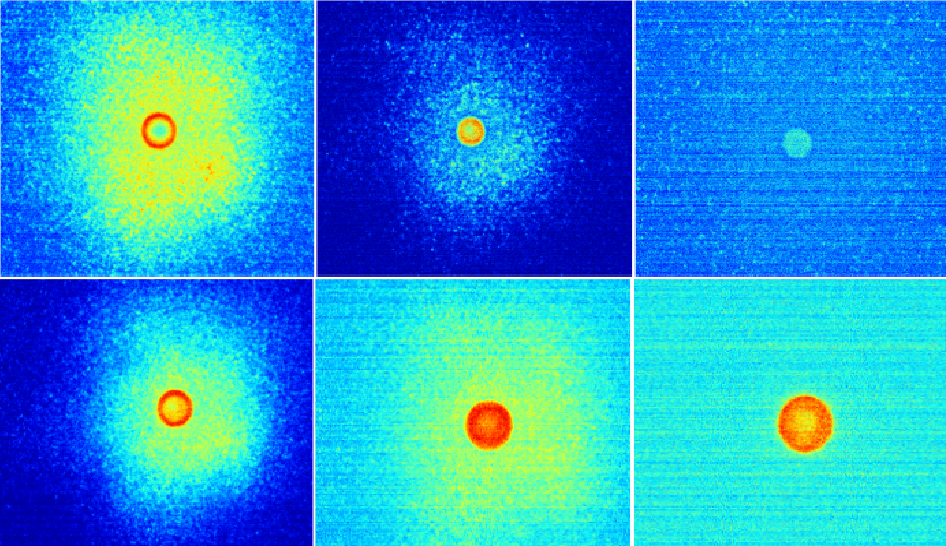
\includegraphics[width=1\textwidth]{../Images/Raw_He_ramdom.png} \end{subfigure} 
\begin{subfigure}[]{0.7\textwidth}
\caption{selected VMI signals for neon in MIR lasers}
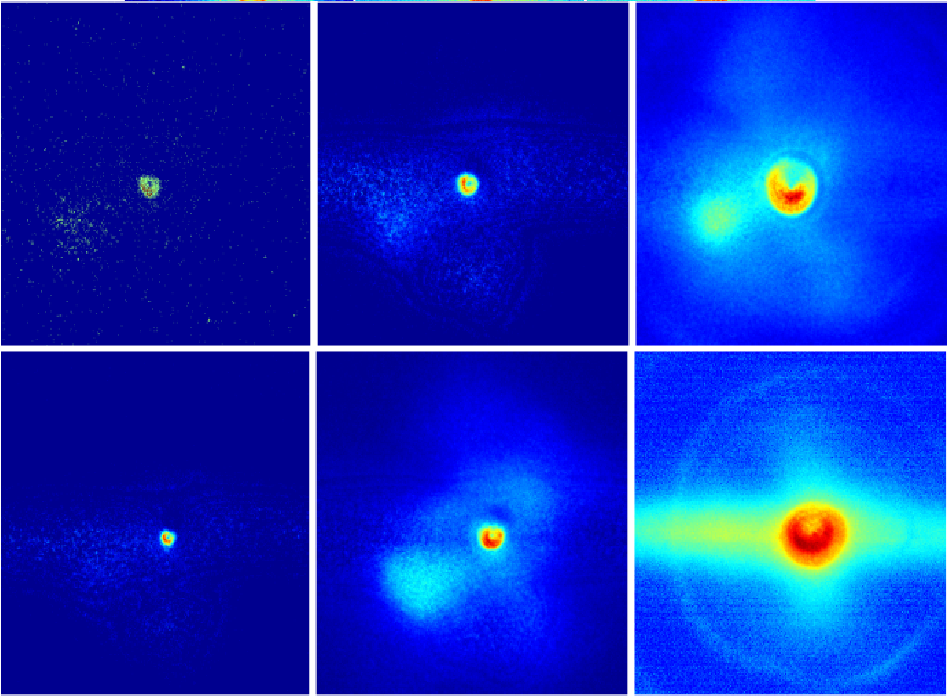
\includegraphics[width=1\textwidth]{../Images/Raw_Ne_ramdom.png} \end{subfigure} 
\caption[VMI raw images example]{Example images of MIR VMI signal in He and Ne with different parameters. On the top, several example plasma signal including, low intensity and the donut shape. On the bottom, random example for Ne signals, including low signal and non-uniform bloops.}
\label{fig:vmiexample}
\end{figure}



\section{Camera and Trigger Protocol}

One of the main objectives of this work was to record single signal for distinct nanoplasma explosion in the VMI and TOF. The ability to treat the data as a individual explosion, reduces the background and makes possible to recall energy distribution information that is lost when data is averaged. With this purpose two methods were developed. 

A first approach was done using a software triggering for the CCD camera in the VMI and the oscilloscope, an Acqiris Card CC103, for the TOF. Using Lab View, an external clock (a RasberryPi 3) is triggered by the laser, considered the beginning of the explosion. At the same time, the laser trigger the camera and the oscilloscope software to start the acquisition. Having all the data acquired in the same program would allow to sort the signals online and reduce the data storage. The Lab view program was tested unsuccessfully for the data acquisition rate of $100$ KHz needed in ELI. The software scheme used applied extra delays due to the communication protocols. Even the data was acquired at the same time, the extra delays used in saving the information it in the hard drive made impossible to correlate the signals.

Based on that same idea, a second approach was used. The laser trigger was connected to a delay generator that at the same time triggers the oscilloscope, a $R.S$ RTO2000 with bandwidth of 600MHZ to 6GHz, and the camera. Two facts need to be taken into account, the minimal exposure time of the camera is 34 $\mu$s and the timing between the camera receiving the trigger signal and the real start of the acquisition is not negligible as it is for the oscilloscope. The camera took 5-6 $\mu$s to start after the trigger was sent. Fig. \ref{fig:triggers} shows the triggering scheme used in the experiment.


\begin{table}[t]

\centering
\begin{tabular}{ll}
\multicolumn{2}{c}{}                                          \\ \hline
\multicolumn{1}{|l|}{Channel} & \multicolumn{1}{l|}{Set to:}    \\ \hline
\multicolumn{1}{|l|}{A}                & \multicolumn{1}{l|}{$T+0$}       \\ \hline
\multicolumn{1}{|l|}{B}                & \multicolumn{1}{l|}{$T+1\mu s$}     \\ \hline
\multicolumn{1}{|l|}{C}                & \multicolumn{1}{l|}{$B$ or B+6 $\mu$s} \\ \hline
\end{tabular}
\caption[trigger Channel delays]{Trigger Channel delays}
\label{tab:delaystriger}
\end{table}

A delay generator (Stanford Research Systems MD DG335) receives the laser trigger (100 KHz), channel B and C were connected to the oscilloscope`s channel 1 and. Channel A was connected to the pin 1 (trigger) of the camera. Due the limitation in the exposure time of the camera, we cannot identify a single laser shot with it. Table \ref{tab:delaystriger} shows the delays used in the experiment, where $T$ is the original laser trigger and A, B and C are the channels in the delay generator. The oscilloscope can identify each individual laser shots but the camera will see at least 3 shots. Fortunately, not all laser shots generates an explosion, meaning that most of the pictures present no signal. Rare cases have the signal of 2 or more explosion and the predominant pictures with signal contain just one explosion in the VMI that can be correlated to its individual TOF signal. 

\begin{figure}[h!]

\centering
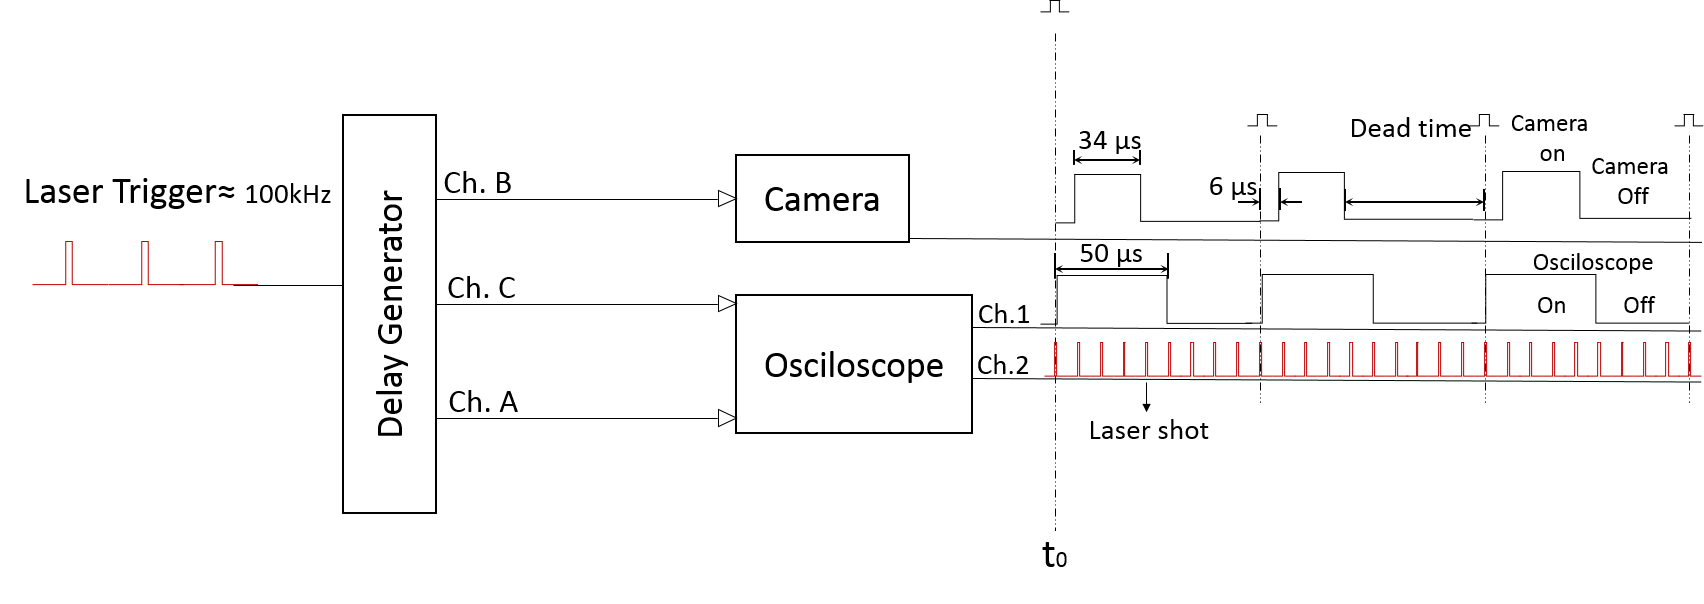
\includegraphics[width = 14 cm]{../Images/Trigger scheme.png}
\caption[Trigger Scheme]{Scheme of the trigger system used to correlate the individual VMI pictures with their corresponding TOF traces }
\label{fig:triggers}
\end{figure}

In Fig \ref{fig:triggers} the oscilloscope and camera are triggered by the delayed channel B. The oscilloscope is set to $50\mu s$ and the camera to the minimal exposure time. The camera and oscilloscope receives the same trigger, the oscilloscope will record at least 5 laser shots, but the camera only record three laser shots. The pictures are saved in the memory RAM of the computer so a dead time after the camera is off is mandatory to give the operating system enough time to save the data on disk. Each of the data sets are saved with a unique label to correlate the signals in the data analysis. Once an explosion is found in the VMI pictures, we check in its corresponding TOF traces that to proof there exist just one explosion in all five laser shots. If just one peak is found, it means the picture correspond to a single Coulomb explosion. In case more than one peak is found, the picture is discarded. 

Fig \ref{fig:correlatesimg} shows an example of some electron-VMI pictures to its corresponding TOF traces. Fig A shows a typical VMI-TOF correlated signals with one peak in the TOF corresponding to He$^{+}$. Fig b. presents a brighter electron VMI picture with a broad He$^+$ yield. Fig c. show an example of a Coulomb explosion where dimmers where formed as show in the TOF with two peaks that correspond to He$^{+}$ and He$^{2+}$.

\begin{figure}[h!]
 \centering
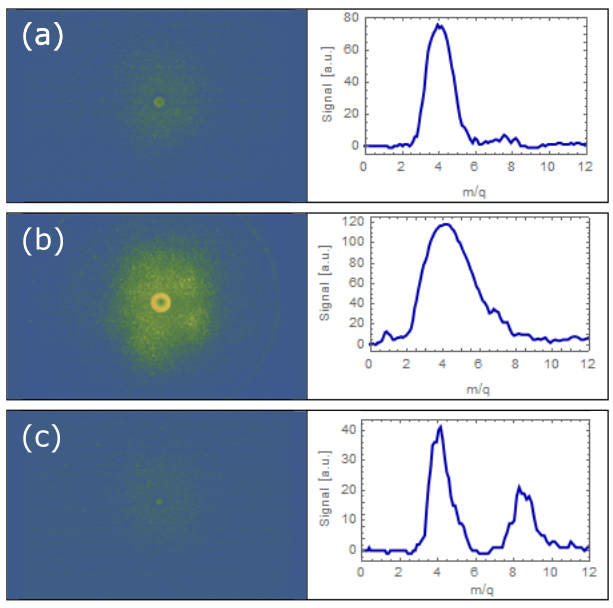
\includegraphics[width=0.6\textwidth]{../Images/results/mir_correlated/mir_correlated.png} 
  \caption[Correlation signals example]{Example of VMI-TOF correlation signals for He droplets. In the left the electron VMI pictures and on the right their correspondent TOF spectra are shown. On the Y-axis the ion yield and on the X-axes the mass/charge ratio is plotted. }
  \label{fig:correlatesimg}
 \end{figure}
  

\section{Calibration Methods}

\subsection{VMI calibration}

To calibrate the VMI spectrometer, two different methods were used. A quadratic calibration function $E=\alpha\cdot r^2$ is used, where $E$ is the kinetic energy of the particles, $r$ is the measured radius and$\alpha$ is thas free parameter is the calibration factor, based on the kinetic energy $E_{kin}=1/2 \cdot m v^2$. In order to keep simplicity, stray fields, third order and linear terms are not included, as long as the calibration curves fit well with the measured data.

The most independent method to calibrate the VMI is using simulate trajectories, because his method does not rely on any laser system or physical process. These simulations were done by Dominik Schomas using SIMION 8.1 software. As starting conditions for the electrons, we chose a small interaction volume comparable to the estimated experimental parameters. The emission direction was set perpendicular to the spectrometer axis. For the electrons in the interaction region, the projected energy on the detector screen is equivalent to the real kinetic energy, so the inverse abel transformation can be avoided. It is necessary to simulate different kinetic energies for the electrons, at different velocity vectors to determine the correct voltages needed in the system and the max energy detected. After extracting the radii, where the electrons hit the detector plane, a calibration from pixels to mm for the camera is needed, because SIMION gives the radii of the electrons in mm. To calibrate pixels to mm the inner diameter of the phosphor scree was used. The disadvantage of this method is, that it is very difficult to include any magnetic or electric stray fields into the simulations or other external parameter that can be fit in a more realistic model.

\begin{figure}[h!]
\centering
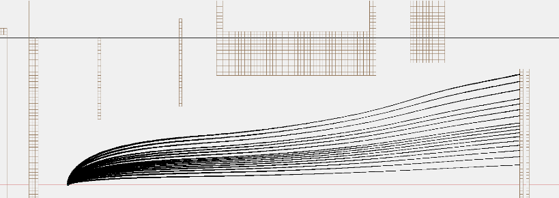
\includegraphics[scale=1]{../images/simion_calib.png}
\caption{energy calibration of the VMI spectrometer with SIMION. Electrons with discrete kinetic energy are emitted perpendicular to the spectrometer axis.}
\end{figure}


Additional to the simulations, a physical process is used to calibrate the VMI. A suitable method to calibrate the spectrometer is create electrons with a well-known energy using above threshold ionization (ATI) of rare gas atoms. The result of the ATI mechanism are several rings in the VMI along the laser polarization axis that are energetically spaced by the energy of one photon. With at least 2 rings visible it is possible to do the calibration with the following formula

\begin{align*}
\Delta E = \alpha (r_2^2-r_1^2)
\end{align*}
where $\Delta E$ is the photon energy, $r_i$ are the peak positions of the Abel inverted rings and $\alpha$ the calibration factor. Best results are achieved by using as low focus intensities as possible, so tunnel ionization is highly suppressed.

A very useful scheme is published by \textit{Wituschek et al.} \cite{wituschek_simple_2016}. The scheme uses continuous 404 nm laser light to excite either the 5p${}_{3/2}$ or the 5p${}_{1/2}$ state in potassium. From this state, relaxation in four other states and the ground state is possible. The 404 nm light can also ionize electrons from the resonant 5p state, the 5s, the 3d and the 4p states. The resulting electrons carry a very well defined kinetic energy $E_{kin}=E_{Photon}+E_{state}-E_{ionization}$. Since all energies on the right side of the equation are well known, the kinetic energy is also well known. This allows the calibration of the spectrometer with three points (the cross section of the 5s state is too small to see it) in the low energy range.
%
%\begin{figure}
%\centering
%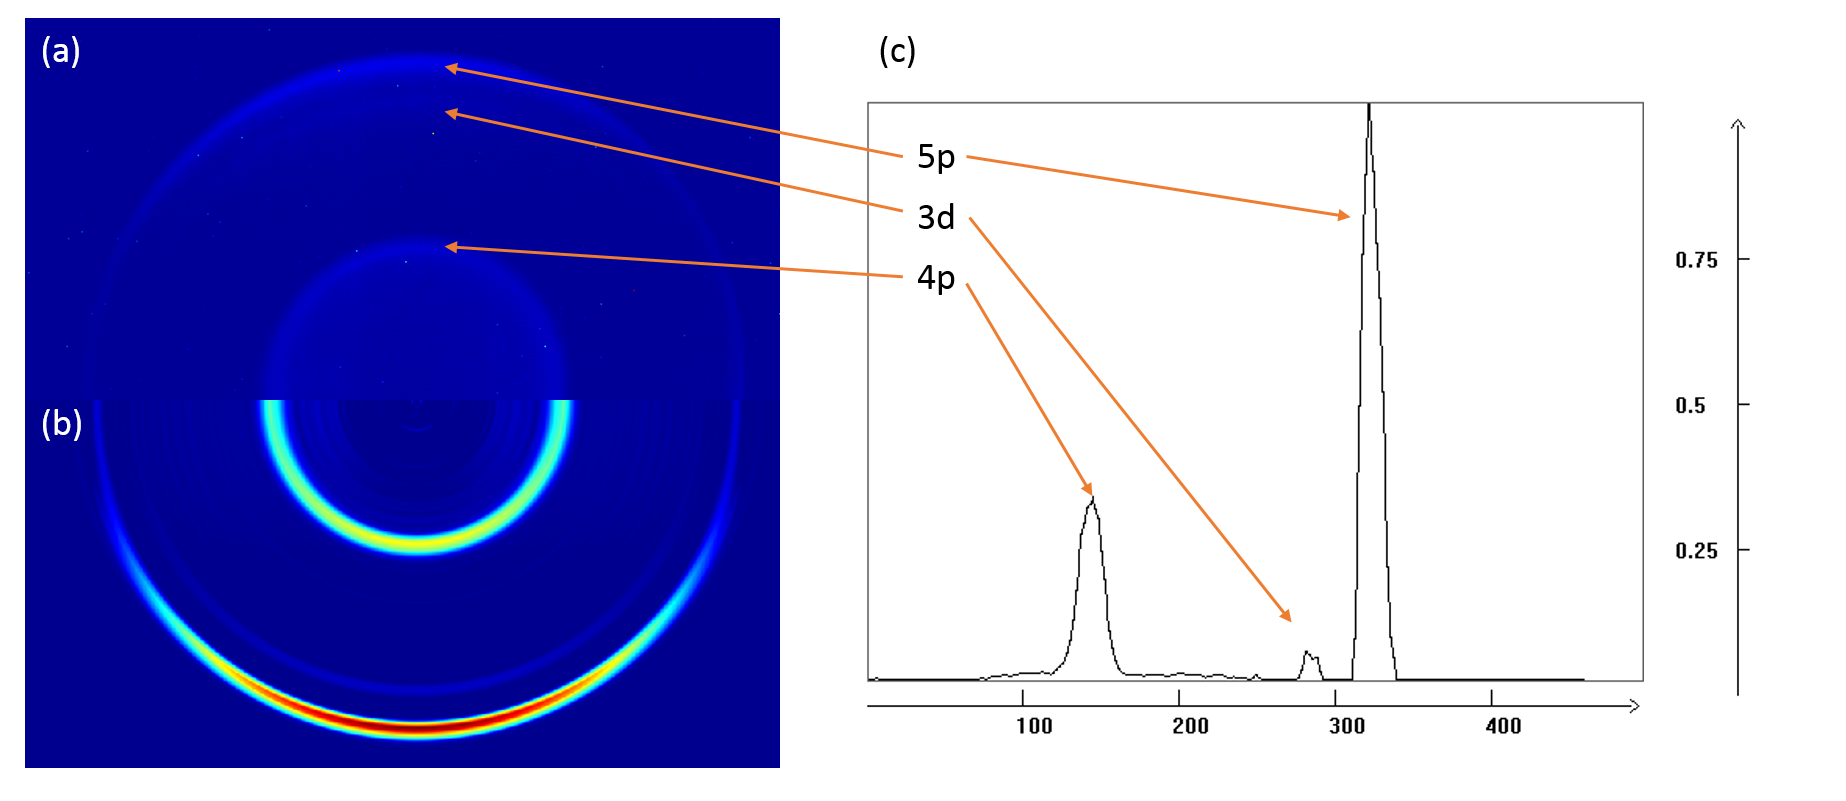
\includegraphics[scale=0.5]{../images/potassium_calib.png}
%\caption{(a) Photoelectron image of potassium excited and ionized by linear polarized 404nm light, (b) Abel inverted image and (c) corresponding photoelectron spectrum, not yet calibrated on the energy}
%\end{figure}


\subsection{Laser Intensity Calibration}
When using a focused MIR and NIR laser, it is essential to know the peak intensity in the focus of the laser field. Most of the time calculations give wrong results, because they assume a perfectly Gaussian shape and do not account losses in optics after the power measurement or an imperfect focus. So it would be desirable to avoid calculations and measure the peak intensity directly. In this thesis two different schemes are used, the 2U$_P$ cutoff energy of electrons in a laser field \cite{becker_vuv_1996} and the ratios of charge states of ions produced in the laser field \cite{augst_laser_1991}.

Assuming that the laser is a perfect Gaussian beams we can calculate using linear optics the focused intensity. In cylindrical coordinates with the origin in the focus of the beam, where z is the direction of propagation and $r$ the distance from the Z-axis. The following equations describes the intensity distribution of a beam:

\begin{equation}
w_{0}=\dfrac{f\lambda}{\pi \omega}
\end{equation}
 where $w_{0}$ is the calculated focus depending on the focal length of the focussed mirror $f$, the wavelength of the laser $\lambda$ and the radius of the collimated beam before it is focused.
the intensity is then given by

\begin{equation}
I_{0}=\dfrac{2P}{\pi \omega_{o}^{2}R \tau}
\end{equation} 
 where $P$ is the power of the laser, $R$ is the repetition rate and $\tau$ is the laser pulse duration.




\section{Data Analysis}

Due the complexity of the Coulomb explosion, few analytical models exist in literature. As shown in Fig. \ref{fig:vmiexample}, the individual signal have a well-defined circular central feature that defers depending on the experiment parameters. Even under the same parameters, the VMI signals continues to have a central circular shape showing different radii and brightens for each single explosion. This central features presents sharp edges and a clearly circular shape that can be advantageous to our analysis. 
Fig. \ref{fig:abeltransf} show a raw picture of single event and its Abel transform. The sharp peak in the electron spectra show the maxima electron kinetic energy, which changes in each explosion. The peak in the energy distribution define the radius of the central with circle, coinciding to the edge of the central feature. Similarly to the results in the Inverse Abel transform for the max kinetic energy in the electrons, we develop a signal finder algorithm to identify the edge of the central circle and its brigtness. In this way, the maximal kinetic energy distribution for a single explosion and its electron yield given by the intensity of the are measured and analyzed.
 
\begin{figure}[h!]
 \centering
 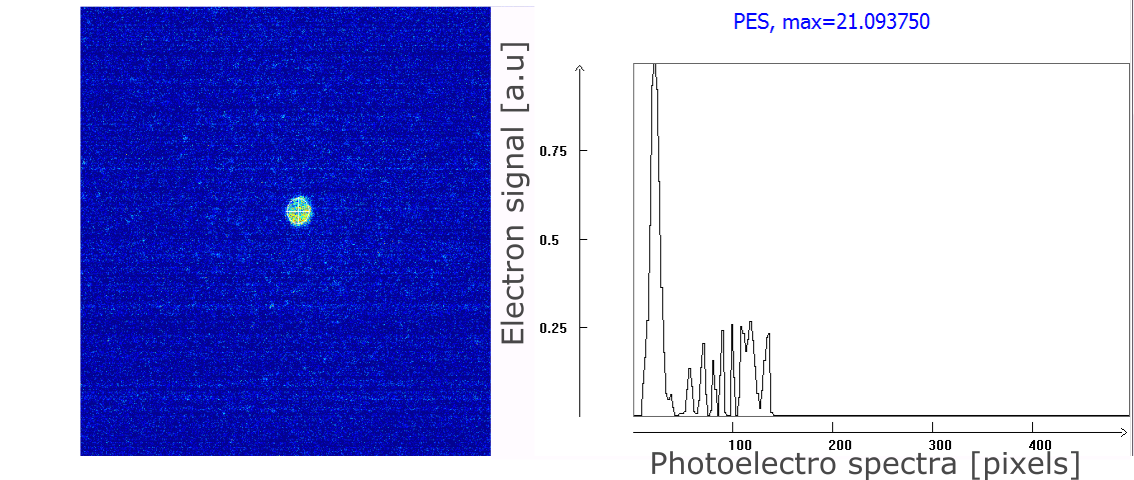
\includegraphics[width=12 cm]{../Images/abel inverse transform.png}
 \caption[Abel inverse transform example]{Example of the Inverse Abel transform for a single shot image. The photo electron spectra show the energy distribution of the signal with a peak in 21 pixels}
 \label{fig:abeltransf}
 \end{figure}

\subsection{Event Recognition}

The low event rate of the nanoplasma explosion results in a lot of empty VMI images. On average 10000 pictures were taken for each data set where less than $10\%$ of them contain signal. To separate empty images from signals, the central bright feature is used. A center for teach data set is selected manually and all pixels within a region around the center are summed up. If the sum is above a certain threshold value the image contains a signal. To analyze the central feature in more detail the size and the brightness of this circle is of importance. Two methods were compared, one using the Mathematica 10.1 (wolfram inc.) algorithms and the other using a binning processing.

First, the ImageMeasurements and Componentmeasurements Mathematica`s functions act over a binarized image. The functions works with arbitrary 2D and 3D images and computes multiple properties, finding components bases on a specific matrix. For this special case, a circular matrix with the specifications of a minimum radius and no share edges were given as parameters. The efficient of this process was demonstrated to depend strongly on the image brightness, the initial binned threshold (BT) and the signal-noise rate. Hence, a recursive function were develop to recursively find an optimal BT so the algorithm find just one object that matches the signal. Once the object is found, the radius and center are saved and the total intensity inside the radius is summed. 

The second method is based on a circular binning of the signal. A center for each data set is manually place after summed all signal pictures. For each individual explosion three circles are defined around this center. The first one with radius $r$ (in pixels), $r$ been variable, the second one with $r_{in} = r-\Delta r$ and the last one with $r_{out} = r + \Delta r$, where $\Delta r$ has to be picked out from the dataset. The three circles define two areas $A_{in}$ and $A_{out}$, see Fig  \ref{fig:density_plot}. An average pixel value $\rho$ for both areas is defined by

\begin{align}
\rho_{in} & = \frac{1}{N_{in}} \sum_{px \in A_{in}} \text{value}(px) - bg \\
\rho_{out} & = \frac{1}{N_{out}} \sum_{px \in A_{out}} \text{value} (px) -bg \\
\end{align}

Where $N$ is the number of pixels in the respective area and $bg$ is a background taken far from the central features. The normalization on the area is important, because the areas are of different size. To finally find out the radius of the central circle, the difference $\rho_{in}-\rho_{in}$ is maximized, this is the case for the orange rig in figure \ref{fig:density_plot}. For the purple ring $\rho_{in} = \rho_{in}$, which gives zero for the difference.
Real signals do not have a perfect cut-off or a constant radial profile, which leads to noisy curves, when $\Delta r$ is chosen too small, it makes the determination of $r$ difficult. An example of a single shot image, where the radius is determined for $\Delta r = 3,4,5$ in pixels, is shown in figure \ref{fig:density_plot} b. 

\begin{figure}
\centering
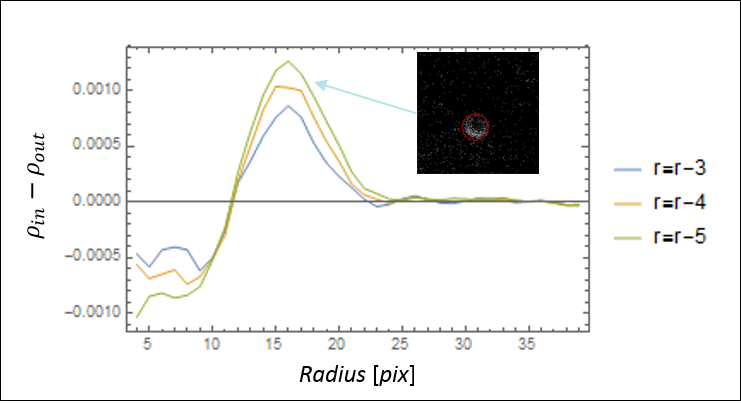
\includegraphics[width=1\textwidth]{../images/density_plot.png}
\caption[Signal finder density plot]{a) radius of the rings used in the signal finder. b) Delta density plot at different $\delta r$. The peak determine the radius of the central feature in the VMI images}
\label{fig:density_plot}
\end{figure}

While rise r, the density difference $\rho_{in} - \rho_{out}$ should remain constant if the density inside the circle is similar. As shown in \ref{fig:density_plot}, the density plot have a summit when the inner or outer density changes signs and two cases are present. First, if the outer density is lower is because $r$ is located in the edge of the central feature. Second, if the inner density is smaller than the outer density it means that an inner less brightest circle exist, present usually in the donut shapes signals. 

Finally, as in the last procedure, the inner pixels in the circle with radius $r$ are summed and the radius-Brightness is save. In the case where an inner circle is clearly identified, the second radius is also saved with its brightness.

Fig \ref{fig:abelfinder} shows a raw image where the inverse Abel transform and the Binned Finder algorithms were compare. The signal shows a clear peak in the photoelectron spectra at 58.6 pixels, while a similar curve is described by the density binned plot of the signal finder algorithm at 60 pix. The two technique shows a good agreements in the recognition of the maximal kinetic energy for VMI signals as shown. On left, the fitted circle for an example image using the signal finder radio. 


\begin{figure}[hbtp!]
\centering
\begin{subfigure}[l]{1\textwidth}
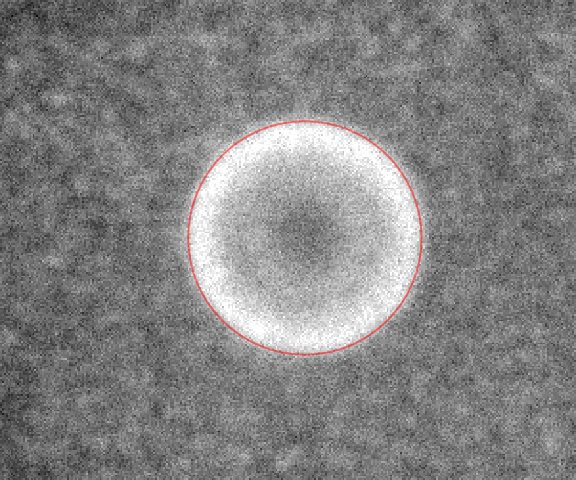
\includegraphics[width=0.4\textwidth]{../Images/rawVMIfit.PNG} 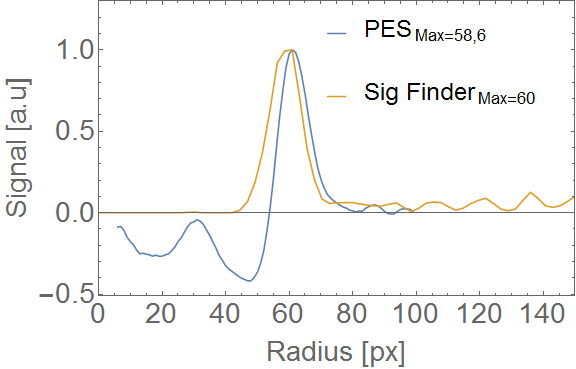
\includegraphics[width=0.5\textwidth]{../Images/pesandFinder.PNG} \end{subfigure} 
\caption[Fit-Abel transform agreement]{On the Left, example images of MIR VMI signal. On the right, the correspond Inverse Abel transform PES (orange) and the Bloop finder density plot (blue). Both algorithms show a peak at radius of the circular signal, highlighted in red. The density plot also shows a second depletion close to 45 pixel that give extra information as the radius of the inner less brighter ring. }
\label{fig:abelfinder}
\end{figure}


\begin{figure}[hbtp]
\caption[Example signal finder]{Example of random signal images fitted to its corresponding radius.}
\centering
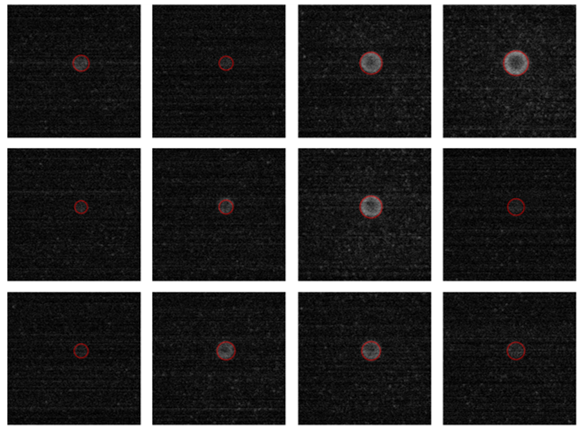
\includegraphics[width=10cm]{../Images/density_plot_chekc.png}
\label{fig:checkradius}
\end{figure}

The calibration factor for the brightness (CFB) is done manually for each data. We search single brighter points in the background cloud, far from the center (to avoid the brightness of the central feature). The CFB correspond to the mean brightness of the identified pixels with a single electron signal. Assuming that pictures are not saturated, the total number of pictures is the total brightness divided the CFB. Finally, from now on for the results, the radius can be converted into maximal kinetic energy, $r\rightarrow E_{max}$, and brightness to number of electrons, $brigt\rightarrow \#e-$. 



